% !TEX root = ../DuvalPeyre-SparseSpikes.tex

%%%%%%%%%%%%%%%%%%%
\section{Discrete Sparse Spikes Deconvolution}
\label{sec-discrete}

  
%%%%%%%%%%%%%%%%%%%%%%%%%%%%%%%%%%%%%%%%%%%%%%%%%%%%%%%%%
\subsection{Finite Dimensional $\ell^1$ Regularization}

A popular way to compute approximate solutions to~\eqref{eq-initial-pb} with fast algorithms is to solve this problem on a finite discrete grid $\Gg\subset \TT$.
Denoting by $P$ the cardinal of the grid $\Gg$, and by $g\in \TT^P$ the finite
 sequence of elements of $\Gg$, the idea is to solve $\Pp_\la(y_0)$ (or~\ref{eq-constrained-pbm})
with the additional constraint that $m=\sum_{i=1}^P a_i \delta_{g_i}$ for some $a\in \RR^P$.

This is nothing but the so-called basis pursuit denoising problem~\cite{chen1999atomi}, also known as the Lasso~\cite{tibshirani1996regre} in statistics.
Indeed, defining the linear operator $\Psi$ through 
\eq{
	\Psi a = \Phi m= \sum_{i=1}^P (\Phi \delta_{g_i})a_i, 
}
the problem amounts to:
\eql{\label{eq-lasso-discr-finite}\tag{$\tilde{\Pp}_\la^\Gg(y_0)$}
	\umin{ a \in \RR^P } \frac{1}{2}\norm{y_0 - \Psi a}^2 + \la \norm{a}_1
	\qwhereq
	\norm{a}_1 = \sum_{i=1}^P |a_i|,
}
where $\Psi:\RR^P \rightarrow L^2(\TT)$ is a linear operator ($L^2(\TT)$ may as well be replaced with $\RR^Q$ or any Hilbert space),
 and $a_i$ denotes the mass at each point $i$ of the grid.
In the noiseless case, the exact reconstruction problem reads:
\eql{\label{eq-lasso-discr-noiseless-finite}\tag{$\tilde{\Pp}_0^\Gg(y_0)$}
 	\umin{ \Psi a = y_0 } \norm{a}_1.
}
The aim of the present section is to study the asymptotic of Problems~\eqref{eq-lasso-discr-finite} and~\eqref{eq-lasso-discr-noiseless-finite} as the stepsize of the grid $\Gg$ vanishes. To this end, we keep the framework of measures and we reformulate the constraint that $\supp(m) \subset \Gg$, i.e. that $m$ can be written as $m=m_{a,x}$, where $x = (x_1,\ldots,x_N)\in \Gg^N$. Recall that the notation $m_{a,x}$ hints that $a_i\neq 0$ for all $i$ and that the $x_i$'s are all distinct, so that in general $N\leq P$. We thus adopt the following penalization term
\begin{align}
	\normTVG{m}= \sup \enscond{ \int \psi \d m }{  
		\psi\in C(\TT), \forall t\in \Gg \ |\psi(t)| \leq 1 },
\end{align}
so that $\normTVG{m}=+\infty$ when $\supp(m) \not\subset \Gg$, and $\sum_{i=1}^N |a_i|$ otherwise.

Problems~\eqref{eq-lasso-discr-finite} and~\eqref{eq-lasso-discr-noiseless-finite} are then respectively  equivalent to:
\eql{\label{eq-lasso-discr}\tag{$\Pp_\la^\Gg(y_0)$}
	\umin{m \in \Mm(\TT)} \frac{1}{2} \norm{\Phi(m) - y_0}^2 + \la \normTVG{m}
}
and 
\eql{\label{eq-lasso-discr-noiseless}\tag{$\Pp_0^\Gg(y_0)$}
	\umin{ \Phi m = y_0 } \normTVG{m},
}


% Gab: removed "may be derived directly in a finite dimensional framework, and more importantly that they"
 
Let us stress the fact that the results of Sections~\ref{subsec-certif-discr} and~\ref{sec-discr-robustness} hold for \textit{any finite dimensional matrix} $\Psi \in \RR^{P \times Q}$ or linear operator $\Psi: \RR^P\rightarrow L^2(\TT)$: the columns of $\Psi$ need not be the samples of a convolution operator. 


%%%%%%%%%%%%%%%%%%%%%%%%%%%%%%%%%%%%%%%%%%%%%%%%%%%%%%%%%
\subsection{Certificates over a Discrete Grid}
\label{subsec-certif-discr}

%\todo{The following notations needed to be introduced somewhere. Check where you want to put it.} 
% Je l'ai mis dans la partie notation
As in Section~\ref{sec-preliminaries}, we may compute the subdifferential of the $\ell^1$ norm. For $m=m_{a,x}=\sum_{i=1}^N a_i\delta_{x_i}$ with support in $\Gg$:
\begin{align}
 	\partial \normTVG{m} = \enscond{\eta\in C(\TT)}{ \norm{\eta}_{\infty,\Gg} \leq 1, 
		\foralls i=1,\ldots,N, \; \eta(x_i)=\sign(a_i) }.
\end{align}
where 
\eq{
	\norm{\eta}_{\infty,\Gg}= \max\enscond{ |\eta(t)| }{ t\in \Gg }.
}


We also introduce the corresponding dual problems:
\eql{\label{eq-initial-dualbisdiscr}\tag{$\Dd_\la^\Gg(y_0)$}
	\umin{ \norm{\Phi^* p}_{\infty,\Gg} \leq 1} \left\|\frac{y_0}{\la}-p\right\|_2^2,
}
\eql{\label{eq-constrained-dualdiscr}\tag{$\Dd_0^\Gg(y_0)$}
	\usup{ \norm{\Phi^* p}_{\infty,\Gg} \leq 1} \dotp{y_0}{p}.
}

\begin{rem}
\label{rem-y-imphi}
Let us denote by $G$ the image by $\Phi$ of all measures with support in $\Gg$.
It may happen (for instance if the grid is too rough) that $y_0\notin G$, in which
 case~\eqref{eq-lasso-discr-noiseless} is not feasible and~\eqref{eq-constrained-dualdiscr} has infinite value. But~\eqref{eq-lasso-discr} is then equivalent to $\Pp_\la^\Gg(y_{0,G})$ where $y_0=y_{0,G}+y_{0,G^\perp}$ is an orthogonal decomposition. 
Problem~\eqref{eq-lasso-discr} is thus an approximation of $\Pp_0^\Gg(y_{0,G})$,
 and the relevant dual problems are $\Dd_\la^\Gg(y_{0,G})$ and $\Dd_0^\Gg(y_{0,G})$.
For the sake of simplicity, we shall assume from now on that $y_0\in G$, but the reader may
keep in mind that this hypothesis
 can be withdrawn by replacing $y$ with $y_{0,G}$.
\end{rem}


In view of Remark~\ref{rem-y-imphi}, we observe that problems~\eqref{eq-initial-dualbisdiscr} and 
\eqref{eq-constrained-dualdiscr} are in fact finite dimensional. Indeed, 
 their constraints being invariant by addition of elements of $G^\perp$,
  we may consider their quotient with the space $G^\perp$.
Therefore the condition $p\in L^2(\TT)$ may be reduced to $p\in G$ where $G$ is a finite dimensional space.

As a consequence, a solution to~\eqref{eq-constrained-dualdiscr} always exists,
 so that we may define the \textit{discrete minimal norm certificate}:
 \begin{align}
	\eta_0^\Gg=\Phi^* p_0^\Gg,&  
	\qwhereq
	p_0^\Gg=\uargmin{p}
		\enscond{ \norm{p}_2 }{ p \mbox{ is a solution of }\eqref{eq-constrained-dualdiscr} }.
\label{eq-min-norm-certifdiscr}
\end{align}
The solutions of~\eqref{eq-lasso-discr} and 
\eqref{eq-initial-dualbisdiscr}
(resp.~\eqref{eq-lasso-discr-noiseless} and~\eqref{eq-constrained-dualdiscr})
are related by the extremality conditions~\eqref{eq-extremal-cdt} (resp.~\eqref{eq-extremal-constrained}) where the total variation is replaced with its discrete counterpart $\normTVG{\cdot}$. 

%%%%%%%%%%%%%%%%%%%%%%%%%%%%%%%%%%%%%%%%%%%%%%%%%%%%%%%%%
\subsection{Noise Robustness}
\label{sec-discr-robustness}

As in the continuous case (cf. Section~\ref{sec-noise-robust}), the support of the solutions of $\Pp_\la^\Gg(y_0+w)$ for $\la \to 0^+$ and $\norm{w}_2=O(\la)$ is governed by the minimal norm certificate. We introduce here the discrete counterpart of the extended support of a measure.

\begin{defn}[Extended support]
Let $m_0\in \Mm(\TT)$ such that $y_0=\Phi(m_0)\in G$, and let $\eta^\Gg_0$ 
be the discrete minimal norm certificate defined in~\eqref{eq-min-norm-certifdiscr}.
 The extended support of $m_0$ relatively to $\Gg$ is defined as
\begin{align}
	\extg(m_0) =\enscond{ t\in \Gg }{ |\eta_0^\Gg(t)|= 1 },
\end{align}
and the extended signed support relatively to $\Gg$ as
\begin{align}
	\extsg(m_0) = \enscond{ (t,v) \in \Gg \times \{-1,+1\} }{ \eta_0^\Gg(t)= v }.
\end{align}
\end{defn}

It is important to notice that the assumption $y_0\in G$ does not mean that the support of $m_0$ is included in $\Gg$, but that there exists  a measure with support included in $\Gg$ which produces the same observation $y_0$. Therefore the support
 of $m_0$ and its extended support may even  be disjoint.
 
As in the continuous case, notice that $m_0$ is a solution of~\eqref{eq-lasso-discr-noiseless}
if and only if $\ssupp(m_0) \subset \extsg(m_0)$.

\begin{thm}[Noise robustness, discrete case]
Let $m_0\in \Mm(\TT)$ such that $y_0=\Phi(m_0)\in G$. Then, there exists $\alpha>0, \la_0>0$,
 such that for $(\la,w) \in D_{\alpha,\la_0}$
 (defined in~\eqref{eq-constr-set}) any solution $\tilde{m}_{\la,w}$ of $\Pp_\la^\Gg(y_0+w)$ satisfies:
\begin{align}
 	\ssupp(\tilde{m}_{\la,w}) & \subset \extsg(m_0).
\end{align}
If, in addition, $\Phi_{\extg(m_0)}$ has full rank and $m_0$ is a solution of~\eqref{eq-lasso-discr-noiseless}, then the solution $\tilde{m}_{\la,w}$ is unique, $m_0$ is identifiable and 
choosing $\la = \norm{w}_2/\al$ ensures $\norm{\tilde{m}_{\la,w}-m}_{2,\Gg} = O(\norm{w})$, where 
\eq{
	\norm{\tilde{m}_{\la,w}-m}_{2,\Gg}^2 = \sum_{x\in \Gg} |m(\{x\})-\tilde{m}_{\la,w}(\{x\})|^2.
}
\label{thm-noise-robustness-discr}
\end{thm}

\begin{proof}
The proof is essentially the same as in the continuous case, therefore we only sketch it. To simplify the notation, we write $J=\extg(m_0)$. The solutions of~\eqref{eq-initial-dualbisdiscr} converge to $p_0^\Gg\in L^2(\TT)$ for $\la \to 0^+$, where $\Phi^*p_0^\Gg=\eta_0^\Gg$ is the discrete minimal norm certificate.

By the triangle inequality
\begin{align*}
\normig{\tilde{\eta}_\la - \eta_0^\Gg}&\leq \underbrace{\normig{\tilde{\eta}_\la-\eta_\la^\Gg}}_{\leq C\frac{\norm{w}_2}{\la} } + \normig{\eta_\la^\Gg-\eta_0^\Gg}
\end{align*}
Thus, there exist two constants $\alpha >0$ and $\la_0>0$, such that for $\frac{\norm{w}_2}{\la}\leq \alpha $ and $0<\la<\la_0$, $|\tilde{\eta}_\la(x)|<1$ for any $x\in \Gg\setminus J$.
Then, the primal-dual extremality conditions imply that for any solution $\tilde{m}_{\la,w}$ of $\Pp_\la^\Gg(y_0+w)$, one has $\supp(\tilde{m}_{\la,w}) \subset J$ and equality of the signs. 

Now, if $\Phi_J$ has full rank, we can invert the extremality condition:
\begin{align*}
	\frac{1}{\la}\Phi_J^* \pa{ 
		y_0 +w - \Phi_J( \restr{\tilde{m}_{\la,w}}{J} ) 
	} 
	&= \restr{\tilde{\eta}_\la}{J},\\
\mbox{so that} \quad \restr{\tilde{m}_{\la,w}}{J} = \restr{m}{J} + \Phi_J^+ w-& \la (\Phi_J \Phi_J^*)^{-1}  \restr{ \tilde{\eta}_\la }{J}.
\end{align*}
Observing that $\normig{ \restr{\tilde{\eta}_\la}{J} }\leq 1$, we obtain the $\ell_2$-robustness result.
\end{proof}

Theorem~\ref{thm-noise-robustness-discr} is analogous to Lemma~\ref{lem-robust-boites} for the continuous problem.
The discrete nature of the problem makes its conclusions more precise.
Although the $\ell^2$-robustness results are similar to those of Theorem~\ref{thm-noise-robustness},
the focus here is a bit more general, in the sense that this theorem does not assert that the
support of the recovered measures matches the support of the input measure $m_0$.
In fact, if $m_0$ is a solution to~\eqref{eq-lasso-discr-noiseless-finite}, $\ssupp(m_0)\subset \extsg(m_0)$, so  that the recovered solutions to $\Pp_\la^\Gg(y_0+w)$ have in general more spikes 
than $m_0$, and the spikes in $\extg(m_0)\setminus \supp(m_0)$ must vanish as $\la\to 0, \norm{w}_2 \to 0$.

In order to get the exact recovery of the signed support for small noise, we may assume in addition that
$\ssupp(m_0)=\extsg(m_0)$ so as to obtain a result analogous to Theorem~\ref{thm-noise-robustness}.
Precisely, we obtain the following theorem which was initially proved by Fuchs~\cite{fuchs2004on-sp}.
First, we introduce a pre-certificate.

\begin{defn}[Fuchs pre-certificate]
Let $m_0 \in \Mm(\TT)$ such that $\supp(m_0)\subset \Gg$. We define the Fuchs pre-certificate as
\begin{align}
\etaF =  \uargmin{\eta =\Phi^* p, p \in L^2} \norm{p}
	\quad\text{subject to}\quad
		\restr{\eta}{\supp m_0} = \sign( \restr{m_0}{\supp m_0}).
\label{eq-fuchs-certif}
\end{align}
\end{defn}
This pre-certificate, introduced in \cite{fuchs2004on-sp}, is a certificate for $m_0$ if and only if $\normig{\etaF} \leq 1$, in which case it is equal to the discrete minimal norm pre-certificate $\eta_0^\Gg$.
 
If $\Phi_{\supp m_0}$ has full rank, then $\etaF$ can be computed by solving a linear system:
\eq{
	\etaF = \Phi^* \Phi_{I}^{+,*} \sign( \restr{m}{I}) 	
	\qwhereq
  I=\supp m_0 
  \qandq \Phi_{I}^{+,*} = \Phi_{I} (\Phi_{I}^*\Phi_{I})^{-1}. 
}

\begin{cor}[Exact support recovery, discrete case,\cite{fuchs2004on-sp}]\label{cor-fuchs}
	Let $m_0 \in \Mm(\TT)$ such that $\supp(m_0) \subset \Gg$, and that $\Phi_{\supp m_0}$ has full rank.
	 If $|\etaF(t)|<1$ for all $t\in \Gg\setminus \supp m_0$,
	  then $m_0$ is identifiable for $\Gg$ and there exists $\alpha>0, \la_0>0$, such that for
	   $(\la,w) \in D_{\alpha,\la_0}$ the solution $\tilde{m}_{\la,w}$ of $\Pp_\la^\Gg(y+w)$
	    is unique and satisfies $\ssupp(\tilde{m})=\ssupp(m_0)$. Moreover 
	\eql{\label{eq-expression-discr-explicit}
		\restr{\tilde{m}_{\la,w}}{I} = \restr{m_0}{I} + \Phi_{I}^+ w - \la (\Phi_{I}\Phi_{I}^*)^{-1} \sign(\restr{m_0}{I}),
	}
  where $I=\supp m_0$.
\end{cor}

The condition $|\etaF(t)|<1$ for all $t\in \Gg\setminus \supp m_0$ is often called the irrepresentability
 condition in the statistics literature, see~\cite{Zhao-irrepresentability}. This condition
  can be shown to be almost a necessary and sufficient condition to ensure exact recovery of
   the support of $m_0$. For instance, if $|\etaF(t)|>1$ for some $t\in \Gg\setminus \supp m_0$,
    one can show that for all $\la > 0$ $\supp(\tilde{m}_\la) \neq \supp m_0$ where $\tilde{m}_\la$ is any
     solution of $\Pp_\la^\Gg(y_0)$, see~\cite{vaiter2011robust}.
In our framework, we see that this irrepresentability condition means that the precertificate $\etaF$
 is indeed a certificate (so that it is equal to the minimal norm certificate), and that its 
saturation set is equal to the support of $m_0$. %When $\etaF$ is not a certificate, this means that $\ssupp(m_0) \neq \extsg(m_0)$
%so that the signed support of $m_0$ is not stable.

For deconvolution problems, an important issue is that Corollary~\ref{cor-fuchs} is
 useless when studying the stability of the original infinite dimensional problem~\eqref{eq-initial-pb}.
  Indeed, the pre-certificate~\eqref{eq-fuchs-certif} is not constrained to have vanishing derivatives,
so that it generally takes some values strictly greater than $1$  for a generic discrete input measure $m_0$.
When the stepsize of the grid is small enough, such values are sampled and $\normig{\etaF}$ necessarily becomes strictly larger than one.
  As detailed in Section~\ref{sec-vanishing}, when shifting from the discrete grid setting
   to the continuous setting, the natural pre-certificate to consider is the vanishing derivative pre-certificate $\etaV$ defined in~\eqref{eq-vanishing-der-certif}, and not the pre-certificate $\etaF$.


%%%%%%%%%%%%%%%%%%%%%%%%%%%%%%%%%%%%%%%%%%%%%%%%%%%%%%%%%%%%%%%%%%%%%%%%%
\subsection{Structure of the Extended Support for Thin Grids}
\label{sec-extended}

In the previous section, we have introduced the notion of extended signed support of a measure $m_0$ relatively to a grid $\Gg$,
and we have proved that this set, $\extsg{m_0}$, contains the  signed supports of all the reconstructed measures for small noise.
In this section, we focus on the structure of the extended support. We show that, if the
 support of $m_0$ belongs to the grid for a sufficiently small stepsize and if the Non Degenerate Source Condition holds,
  the extended signed support consists in the signed support of $m_0$ and possibly one immediate neighbor with the same sign for each spike. 
Therefore, when the grid stepsize is small enough, the support of the measure is generally not stable
for the discrete problem, but the support of the reconstructed measure is a close approximation
 of the original one.

From now on, for the sake of simplicity, we consider dyadic grids $\Gg_n=\enscond{ \frac{j}{2^n} }{�0\leq j \leq 2^n-1 }$. The constraint sets in $\Dd_\la^{\Gg_n}(y_0)$ and~\eqref{eq-initial-dual} are denoted respectively by
\begin{align}
	C_n&=\enscond{ p\in L^2(\TT) }{
		 \left|(\Phi^*p)\left(\frac{j}{2^n}\right)\right|\leq 1,\ 0\leq j\leq 2^n }, \\
	\mbox{and }
	C &= \enscond{ p\in L^2(\TT) }{
			\left\|\Phi^*p\right\|_{\infty}\leq 1
		}
		= \bigcap_{n\in \NN} C_n.
\end{align}


The structure of $\extsg(m_0)$ for large $n$ is intimately related to the convergence of $p^{\Gg_n}_0$ to $p_0$. First, let us notice the following result, whose proof is given in Appendix~\ref{sec-proof2}.

\begin{prop}[Convergence for fixed $\la$]
Let $m_0\in \Mm(\TT)$. Then, for any $\la >0$,
\begin{align}
 \lim_{n\to +\infty} p_\la^{\Gg_n}&= p_\la \mbox{ for the } L^2(\TT) \mbox{(strong) topology},\\
\mbox{ and } \lim_{n\to +\infty} \eta_\la^{\Gg_n}&= \eta_\la \mbox{ for the topology of the uniform convergence}.
\end{align}
Moreover, if there exists a solution to the continuous dual problem~\eqref{eq-constrained-dual},
\begin{align}
 \lim_{\la \to 0^+} \lim_{n\to +\infty} p_\la^{\Gg_n}= p_0, \mbox{ and } \lim_{\la \to 0^+} \lim_{n\to +\infty} \eta_\la^{\Gg_n}= \eta_0. 
 \label{eq-double-limite}
\end{align}
\label{prop-cv-fixedla}
\end{prop}

Proposition~\ref{prop-cv-fixedla} simply states that the projection onto convex sets $C_n$ which
converge (in the sense of set convergence) to $C$ converges to the projection onto $C$. However, 
the case $\la=0$ is not as straightforward, and for instance one cannot easily swap the limits in~\eqref{eq-double-limite}.
In fact, given any decreasing sequence of polyhedra $C_n$, it is not true in general that 
the minimal norm solution of $\sup_{p\in C_n} \dotp{y_0}{p}$ should converge to
the minimal norm solution of  $\sup_{p\in C} \dotp{y_0}{p}$ where $C=\bigcap_{n\in \NN}C_n$.
 As a consequence it is not clear to us whether this convergence always holds for polyhedra of the form 
\eq{
 	C_n = \enscond{ p\in L^2 }{�\norm{\Phi^*p}_{\infty,\Gg_n}\leq 1 }.
}

However, when the spikes locations belong to the grid for $n$ large enough, the convergence of the minimal norm certificates holds.
In the case of dyadic grids, this is equivalent to $m_0\in \Mm(\TT)$ being a \textit{discrete dyadic measure}, i.e. such that for some $n_0\in \NN$:
\begin{align}
	m = \sum_{i=1}^N a_{i} \delta_{x_{i}}, 
	\qwithq 
	x_i=\frac{j_i}{2^{n_0}} \mbox{ and } 0\leq j_i \leq 2^{n_0}-1.
\label{eq-dyadic-measure}
\end{align}

The proofs given below make use of a remark given in~\cite{Candes-toward}: if a solution of the continuous problem~\eqref{eq-constrained-pbm} has support in the grid $\Gg$, then it is also a solution of the discrete problem~\eqref{eq-lasso-discr-noiseless}.


\begin{prop}[Convergence for dyadic measures]
Let $m_0\in \Mm(\TT)$ be a discrete dyadic measure (see~\eqref{eq-dyadic-measure}), and assume
 that the (possibly degenerate) source condition holds. Then
\begin{align}
\lim_{n\to +\infty} p_{0}^{\Gg_n}&=p_0 \mbox{ for the } L^2 \mbox{ (strong) topology},\\
\mbox{and }\lim_{n\to +\infty} \eta_{0}^{\Gg_n(i)}&=\eta_0^{(i)} \mbox{ for } 0\leq i \leq 2, \mbox{ in the sense of the uniform convergence,}
\end{align}
where $\eta_0 = \Phi^* p_0$ (resp. $\eta_{0}^{\Gg_n}=\Phi^* p_{0}^{\Gg_n}$) denotes the corresponding minimal norm certificate.
\label{prop-cv-dyadic}
\end{prop}

\begin{proof}
First, following~\cite{Candes-toward}, we observe that, since $(\Phi^*p_0)(x_i)=\sign(a_i)$ and $\normi{\Phi^*p_0} \leq 1$ (a fortiori $|\Phi^*p_0\left(\frac{j}{2^n}\right)|\leq 1$ for $1\leq j\leq 2^n-1$),
$\Phi^*p_0$ is also a dual certificate for~$(\Pp_0^{\Gg_n})$ provided $n\geq n_0$. As a consequence $\norm{p_{0}^{\Gg_n}}_2\leq \norm{p_0}_2$.

The sequence $(p_{0}^{\Gg_n})_{n\in \NN}$ being bounded in $L^2(\TT)$, we may extract a subsequence (still denoted by $p_{0}^{\Gg_n}$) 
 which weakly converges to some $\tilde{p}\in L^2(\TT)$, and
\begin{align}
 	\norm{\tilde{p}}_2 \leq \liminf_{n\to +\infty} \norm{p_{0}^{\Gg_n}}_2 
	\leq \limsup_{n\to +\infty} \norm{p_{0}^{\Gg_n}}_2 \leq \norm{p_0}_2.
 	\label{eq-limsup-norm}
\end{align}
Moreover, by optimality of $p_{0}^{\Gg_n}$ for the discrete problem, for each $p\in C\subset C_n$,
 $\dotp{y_0}{p_{0}^{\Gg_n}} \geq \dotp{y_0}{p}$ so that in the limit $\dotp{y_0}{\tilde{p}} \geq \dotp{y_0}{p}$.
Observing that $\tilde{p}\in C=\bigcap_{n\in \NN}{C_n}$ (since each $C_n$ is
  weakly closed) we conclude that $\tilde{p}=p_0$. Since the limit does not depend on the extracted subsequence,
  we conclude that the whole sequence $(p_0^{\Gg_n})_{n\in \NN}$ converges to $p_0$, and equality in~\eqref{eq-limsup-norm}
  implies that the convergence is strong.

The consequence regarding $\eta_{0}^{\Gg_n}$ is straightforward.
\end{proof}

We may now describe the structure of the extended support for dyadic measures which satisfy the Non Degenerate Source Condition.

\begin{prop}[Extended support]
Let $m_0=\sum_{i=1}^N a_i \delta_{x_i}$ be a discrete dyadic measure which satisfies the Non Degenerate Source Condition.
Then, for $n$ large enough, there exists $\varepsilon^n \in \{+1,-1\}^N$
such that:
\begin{align}
\ssupp(m_0) \subset \exts_{\Gg_n}(m_0) \subset \ssupp(m_0) \cup \left(\ssupp(m_0) + \frac{\varepsilon^n}{2^n} \right), 
\end{align}
where $\ssupp(m_0) + \frac{\varepsilon^n}{2^n}= \enscond{ (x_i+\frac{\varepsilon^n_i}{2^n},\eta_{0}^{\Gg_n}(x_i)) }{ 1\leq i\leq N }$.
\label{prop-extsupp}
\end{prop}

\begin{cor}
Under the hypotheses of Proposition~\ref{prop-extsupp}, for $n$ large enough, there exist two constants $\alpha(n)>0$
 and $\lambda_0(n)>0$ such that, for $\frac{\norm{w}_2}{\la}<\alpha(n)$ and  $0<\la <\la_{0}(n)$,
 any solution $\tilde{m}_\la^{\Gg_n}$ of $(\Pp_\la^{\Gg_n})$ has support in $\{ x_i,\ 1\leq i\leq N\} \cup \{x_i+\frac{\varepsilon^n_i}{2^n}, \ 1\leq i\leq N \}$, with signs $\eta_{0}^{\Gg_n}(x_i)$, $1\leq i\leq N$.
\label{cor-extended-support}
  \end{cor}
    
  \begin{proof}[Proof of Proposition~\ref{prop-extsupp}]
We describe the points where the value of $\eta_0^{\Gg_n}$ may be $\pm 1$.
By the Non-Degenerate Source Condition, there exists $\epsilon>0$ small enough such that
 the intervals $(x_{0,i}-\epsilon, x_{0,i}+\epsilon)$, $1\leq i\leq N$, do not intersect,
 and that for all $t\in \bigcup_{i=1}^N (x_{i}-\epsilon, x_{i}+\epsilon)$, $|\eta_0(t)|\geq C>0$ and $|\eta_0''(t)|\geq C>0$.
Moreover, $\sup_{K_\epsilon} |\eta_0| <1$ with $K_\epsilon = \TT\setminus \bigcup_{i=1}^N (x_{i}-\epsilon, x_{i}+\epsilon)$.
 
 Therefore, by Proposition~\ref{prop-cv-dyadic}, for $n$ large enough: 
 \begin{itemize}
 \item $|\eta_{0}^{\Gg_n}(t)|\geq \frac{C}{2}>0$ for $t\in (x_{i,0}-\varepsilon,x_{i,0}+\varepsilon)$,
 \item $|(\eta_{0}^{\Gg_n})''(t)|\geq \frac{C}{2}>0$ for $t\in (x_{i}-\varepsilon,x_{i}+\varepsilon)$,
 \item $\sup_{K_\epsilon} |\eta_{0}^{\Gg_n}| <1$,
 \end{itemize} 
and in each interval $(x_{i,0}-\varepsilon,x_{i}+\varepsilon)$, $\eta_{0}^{\Gg_n}$ has the same sign as $\eta_{0}$
 and it is strictly concave (resp. strictly convex) if $\eta_0(x_i)=1$ (resp. $-1$).
  
Assume for instance that $\eta_0(x_i)=1$. The extremality conditions between $p_0$ and $m_0$ for $(\Pp_0(y))$ also imply that 
$m_0$ is a solution of~$(\Pp_0^{\Gg_n}(y_0))$. Then, the extremality conditions
 between $p_{0}^{\Gg_n}$ and $m_0$ imply that $\eta_{0}^{\Gg_n}(x_{i})=1$ as well.
By the strict concavity of $\eta_{0}^{\Gg_n}$ there is at most one other point $t^\star\in (x_{i}-\varepsilon,x_{i}+\varepsilon)$
 such that $\eta_{0}^{\Gg_n}(t^\star)=1$, and since $\eta_{0}^{\Gg_n}(x_{i}\pm \frac{1}{2^n})\leq 1$, $|t^\star-x_i|\leq \frac{1}{2^n}$.
Such a point $t^\star$ contributes to the extended support of $m$ if and only if it belongs to the grid (i.e. $t^\star=x_i\pm \frac{1}{2^n}$).

The argument for $\eta_0(x_i)=-1$ is similar. This concludes the proof.
  \end{proof}

Corollary~\ref{cor-extended-support} highlights the difference between the continuous and 
the discretized problems. In the first case,
any small noise would induce a slight perturbation of the spikes locations and amplitudes,
 but their number would stay the same. In the second case, the spikes cannot ``move'', so that
 new spikes may appear, but only at one of the immediate neighbors of the original ones.

For non-dyadic measures, we may show using Proposition~\ref{prop-cv-fixedla} that for small,
 fixed $\la >0$, and $n$ large enough, there is at most one pair of spikes (located at
  consecutive points of the grid) in the neighborhood
  of each original spike. From our numerical experiments described below (in the case of the ideal low-pass filter),
 we conjecture that, in the case where there are indeed two spikes, they surround the location of the original spike.


\subsection{Application to the Ideal Low-pass Filter}


To conclude this section, we compare the different (pre-)certificates involved in the above discussion,
 whether on the discrete grid or in the continuous domain. 
Then we illustrate the convergence of the sets $(C_n)_{n\in \NN}$ towards $C$.

\paragraph{Certificates.}
Figure~\ref{fig-certif-grid} illustrates the results of Section~\ref{sec-extended}.
The numerical values are $f_c=6$, $n=7$, and the distance between the two opposite spikes is $\frac{0.6}{f_c}$.
The continuous minimal norm certificate $\eta_0$ is shown: it satisfies $|\eta_0(t)|\leq 1$
 for all $t\in \TT$ and $\eta_0(x_i)=\sign m_0(\{x_i\})$ for $1\leq i\leq N$. The discrete
  minimal norm certificate $\eta_0^{\Gg_n}$ satisfies $|\eta_0^{\Gg_n}(t)|\leq 1$
 for all $t$ in the grid, and $\eta(u)=\sign m_0(\{x_i\})$ for all $u\in\ext_{\Gg_n}$
in the neighborhood of $x_i$. For a dyadic measure, such points are $x_i$ and possibly one of its immediate neighbors.
 For non dyadic measures, we conjecture that such points are the two immediate neighbors of $x_i$.

The Fuchs precertificate $\etaF$ is also shown. Some points $t$ of the grid do not satisfy $|\etaF(t)|\leq 1$, hence the Fuchs pre-certificate is not a certificate and the support is not stable. This was already clear from the fact that $\supp(m_0) \subsetneq \ext_{\Gg_n}(m_0)$.

\begin{figure}[htbp]
\centering
\setcounter{subfigure}{0}
\subfloat[Dyadic measure]{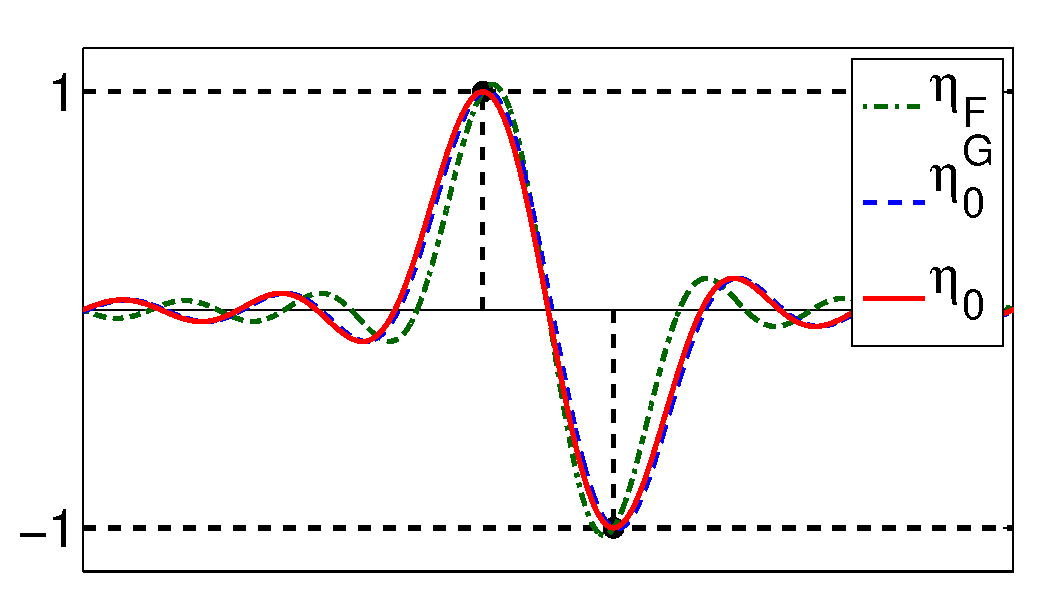
\includegraphics[width=0.47\linewidth] {discrete/ideal-2diracsa-80-ongrid1}}
\subfloat[Non dyadic measure]{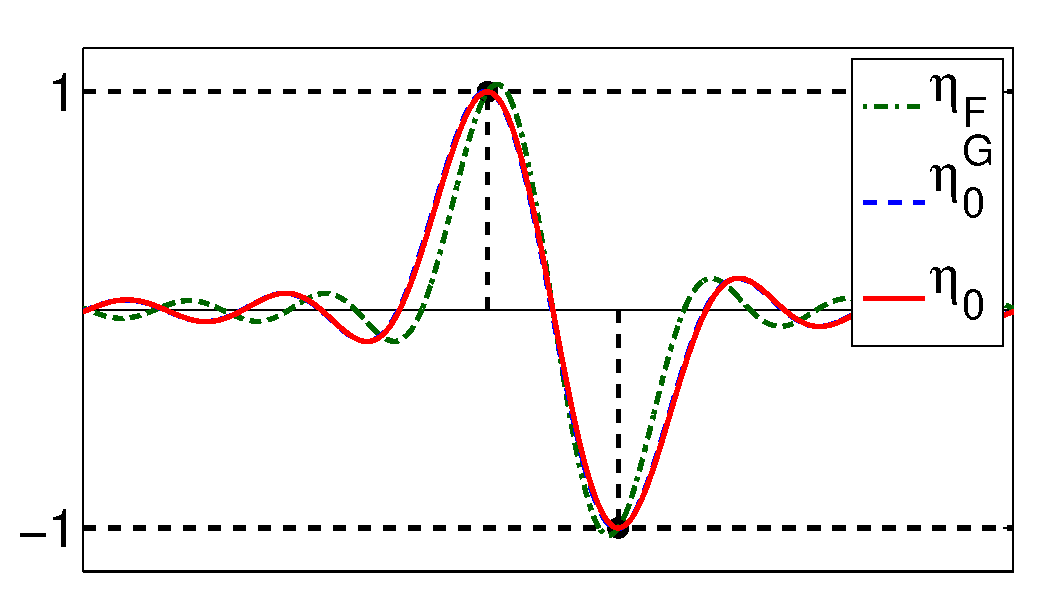
\includegraphics[width=0.47\linewidth] {discrete/ideal-2diracsa-80-ongrid0}}\\
\subfloat[Zoom]{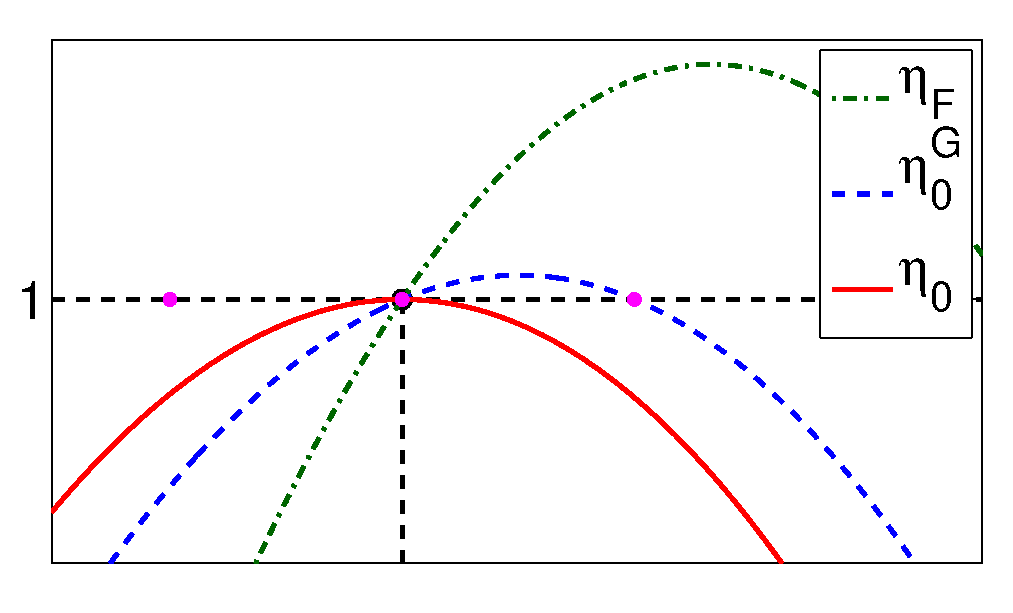
\includegraphics[width=0.45\linewidth] {discrete/ideal-2diracsa-80-ongrid1-zoom}}
\hspace{2mm}\subfloat[Zoom]{\includegraphics[width=0.45\linewidth] {discrete/ideal-2diracsa-80-ongrid0-zoom}}\\
\caption{\label{fig-certif-grid} Comparison of certificates for a dyadic (left) and a non-dyadic measure (right).
The second row is a zoom of the first one near the left spike.
The (continuous) minimum norm certificate $\eta_0$ (in continuous red line) is everywhere bounded by $1$.
The (discrete) minimum norm certificate $\eta_0^{\Gg_n}$ (in dashed blue line) is bounded by $1$ at the grid points.
The Fuchs pre-certificate $\etaF$ (dash-dot green line) is above $1$ at some points of the grid: the Fuchs criterion is not satisfied.
}
\end{figure}

Figure~\ref{fig-coeff-grid} focuses on the reconstructed amplitudes $\tilde{a}_i$ using $\Pp_\la(y_0)$ as $\la \to 0$. Each curve represents a path $\la \mapsto \tilde{a}_i$. Note that for the problem on a finite grid, such paths are piecewise affine. In the dyadic case (left part of the figure), the amplitude at $x_i$ (continuous line) and at the next point of the grid (dashed line) are shown.
As $\la \to 0$, the spike at the neighbor vanishes and the result tends to the original
 identifiable measure.
In the non dyadic case (right part of the figure), the amplitude at the two immediate neighbors of $x_i$ are shown (continuous and dashed lines).
Here $\supp m_0 \not\subset \Gg$ so that $m_0$ is not identifiable for the discrete problem.
For each spike, the amplitudes of the two neighbors converge to some non zero value. The limit measure as $\la \rightarrow 0$ is the solution of $\Pp_0(y_{0G})$.


\begin{figure}[htbp]
\centering
\subfloat[Dyadic measure]{\includegraphics[width=0.48\linewidth] {discrete/ideal-2diracsa-80-ongrid1-path}}
\subfloat[Non dyadic measure]{\includegraphics[width=0.48\linewidth] {discrete/ideal-2diracsa-80-ongrid0-path}}
\caption{\label{fig-coeff-grid} 
Display of the solution path (as a function of $\la$) for the measure displayed on Figure~\ref{fig-certif-grid}. 
Left: Amplitudes of the coefficients at $x_i$ (continuous line) and at the next point of the grid (dashed line) as $\la$ varies.
Right: idem for the two immediate neighbors of $x_i$. 
Some other spikes (grey continuous line) appear and vanish before the last segments, as $\la \to 0$.}
\end{figure}

\paragraph{Set convergence.} Now, we interpret the convergence of the discrete problems
 through the convergence of the corresponding constraint set for the dual problem.
Writing $\Phi^* p(x)=\int p(t)\phi(x-t) \d t= \dotp{p}{\phi_x}_{L^2}$ with $\phi_x : t\mapsto \phi(x-t)$,
 we observe that:
\begin{align}
 	C_n &= \enscond{ p\in \Im \Phi }{
 		\left|\Phi^*p \left(\frac{j}{2^n}\right)\right|\leq 1, \ 0\leq j \leq 2^n-1
	}\\
 		&= \enscond{p\in \Im \Phi }{ 
		|\dotp{p}{\phi_{\frac{j}{2^n}}}_{L^2}| \leq 1, \ 0 \leq j \leq 2^n-1
	}.
 \end{align}
 As a consequence $C_n$ is the polar set of the convex hull of 
$\enscond{ \pm \phi_{\frac{j}{2^n}} }{ 0\leq j \leq 2^n-1 }$.

In the case of the Dirichlet kernel, the vector space $\Im \Phi$ is the space of trigonometric polynomials with degree less than or equal to $f_c$.
An orthonormal basis of $\Im \Phi$ is given by: $(c_0,c_1,\ldots c_{f_c}, s_1, \ldots s_{f_c})$ where 
$c_0 \equiv 1$, $c_k: t\mapsto \sqrt{2}\cos (2\pi kt)$ and $s_k: t\mapsto \sqrt{2}\sin (2\pi kt)$ for $1\leq k\leq f_c$.


Moreover,
\begin{align*}
\phi(x-t)&= \frac{1}{2f_c+1}\left(1+\sum_{k=1}^{f_c} 2\cos (2\pi k (x-t))\right)\\
&= \frac{1}{2f_c+1}\left(1+2\sum_{k=1}^{f_c} \left(\cos (2\pi kx) \cos(2\pi kt) +\sin (2\pi kx)\sin (2\pi kt) \right)\right)
\end{align*}
so that we may write:
\begin{align*}
\phi_x=\frac{1}{2f_c+1}\left(c_0+\sqrt{2}\sum_{k=1}^{f_c}\left(\cos (2\pi kx) c_k + \sin (2\pi kx)s_k \right)\right).
\end{align*}

\begin{figure}[htbp]
\centering
\subfloat{\includegraphics[width=0.30\linewidth,clip=true,trim=90px 40px 90px 40px]{convexe-n3}}\hfill
\subfloat{\includegraphics[width=0.30\linewidth,clip=true,trim=90px 40px 90px 40px]{convexe-n4}}\hfill
\subfloat{\includegraphics[width=0.30\linewidth,clip=true,trim=90px 40px 90px 40px]{convexe-n7}}\\    \setcounter{subfigure}{0}
\subfloat[$C_3$]{\includegraphics[width=0.30\linewidth,clip=true,trim=90px 40px 90px 40px]{convexe-n3bis}}\hfill
\subfloat[$C_4$]{\includegraphics[width=0.30\linewidth,clip=true,trim=90px 40px 90px 40px]{convexe-n4bis}}\hfill
\subfloat[$C_7$]{\includegraphics[width=0.30\linewidth,clip=true,trim=90px 40px 90px 40px]{convexe-n7bis}}\\
\caption{\label{fig-convexe} Top: The convex set $C_n$ for $f_c=1$, and $n=3$, $4$ or $7$ (from left to right).
Bottom: same convex sets, the red spheres indicate the (rescaled) vectors $\phi_{\frac{j}{2^n}}$. }
\end{figure}

For $f_c=1$, we obtain $\phi_x=\frac{1}{3}\left(c_0+\sqrt{2}\left(\cos (2\pi x) c_1 + \sin (2\pi x)s_1 \right)\right)$, and the vectors $\phi_x$ lie on a circle. The convex hull of $\enscond{ \pm \phi_{\frac{j}{2^n}} }{ 0\leq j \leq 2^n-1 }$
 is thus a cylinder, and its polar set $C_n$ is displayed in Figure~\ref{fig-convexe} for $n=3$, $4$, and $7$.

Problem~$(\Dd_\la^{\Gg_n}(y_0+w))$ corresponds to the projection of $\frac{y_0+w}{\la}$ onto the polytope $C_n$. Each face of $C_n$ corresponds to a possible signed support of the solutions $\tilde{m}_{\la,w}$. The large, flat faces of $C_n$ yield stability to the support of $\tilde{m}_{\la,w}$ for
 small noise $w$, as described by Theorem~\ref{thm-noise-robustness-discr}. As $n\to +\infty$ 
these faces converge into a piecewise smooth manifold and the support of $\tilde{m}_{\la,w}$
 is allowed to vary smoothly in $\TT$, according to Theorem~\ref{thm-noise-robustness}.







